\subsection*{Problema 12}

\textbf{Enunciado:} \\
Calcular la integral indefinida:
\begin{align*}
\int \dfrac{\sec x \, dx}{\sec x + 2\tan x - 1}
\end{align*}

\textbf{Solución:} \\
Siguiendo la indicación, expresamos las funciones trigonométricas en términos de $\sin x$ y $\cos x$:
\begin{align*}
\sec x &= \dfrac{1}{\cos x}, \quad 
\tan x = \dfrac{\sin x}{\cos x}
\end{align*}

Sustituimos estas expresiones en el integrando:
\begin{align*}
\int \dfrac{\dfrac{1}{\cos x}}{\dfrac{1}{\cos x} + \dfrac{2\sin x}{\cos x} - 1} \, dx
\end{align*}

Multiplicamos el numerador y el denominador por $\cos x$ para simplificar la fracción compleja:
\begin{align*}
\int \dfrac{1}{1 + 2\sin x - \cos x} \, dx
\end{align*}

Aplicamos la sustitución universal de Weierstraß, definida como $z = \tan\left(\dfrac{x}{2}\right)$. 
De esta sustitución se obtienen las siguientes equivalencias trigonométricas y diferenciales:
\begin{align*}
\sin x &= \dfrac{2z}{1 + z^2}, \quad 
\cos x = \dfrac{1 - z^2}{1 + z^2}, \quad
dx = \dfrac{2 \, dz}{1 + z^2}
\end{align*}

Sustituimos $z$ y $dx$ en la integral:
\begin{align*}
\int \dfrac{1}{1 + 2\left(\dfrac{2z}{1 + z^2}\right) - \left(\dfrac{1 - z^2}{1 + z^2}\right)} \cdot \dfrac{2 \, dz}{1 + z^2}
\end{align*}

Simplificamos el denominador común en la fracción:
\begin{align*}
1 + \dfrac{4z}{1 + z^2} - \dfrac{1 - z^2}{1 + z^2} &= \dfrac{(1 + z^2) + 4z - (1 - z^2)}{1 + z^2} \\
&= \dfrac{2z^2 + 4z}{1 + z^2}
\end{align*}

Reemplazamos este resultado en la integral:
\begin{align*}
\int \dfrac{1}{\dfrac{2z^2 + 4z}{1 + z^2}} \cdot \dfrac{2}{1 + z^2} \, dz &= \int \dfrac{1 + z^2}{2z^2 + 4z} \cdot \dfrac{2}{1 + z^2} \, dz \\
&= \int \dfrac{2}{2z(z + 2)} \, dz \\
&= \int \dfrac{1}{z(z + 2)} \, dz
\end{align*}

Descomponemos el integrando en fracciones parciales:
\begin{align*}
\dfrac{1}{z(z + 2)} &= \dfrac{A}{z} + \dfrac{B}{z + 2} \\
1 &= A(z + 2) + Bz
\end{align*}

Evaluando para $z = 0$ obtenemos $A = \dfrac{1}{2}$, y para $z = -2$ obtenemos $B = -\dfrac{1}{2}$. 
La integral se reescribe como:
\begin{align*}
\int \left( \dfrac{1/2}{z} - \dfrac{1/2}{z + 2} \right) dz &= \dfrac{1}{2} \ln|z| - \dfrac{1}{2} \ln|z + 2| + C \\
&= \dfrac{1}{2} \ln\left| \dfrac{z}{z + 2} \right| + C
\end{align*}

Regresando a la variable original $x$ mediante $z = \tan\left(\dfrac{x}{2}\right)$:
\begin{align*}
F(x) = \dfrac{1}{2} \ln\left| \dfrac{\tan\left(\dfrac{x}{2}\right)}{\tan\left(\dfrac{x}{2}\right) + 2} \right| + C
\end{align*}

\begin{figure}[H]
	\centering
	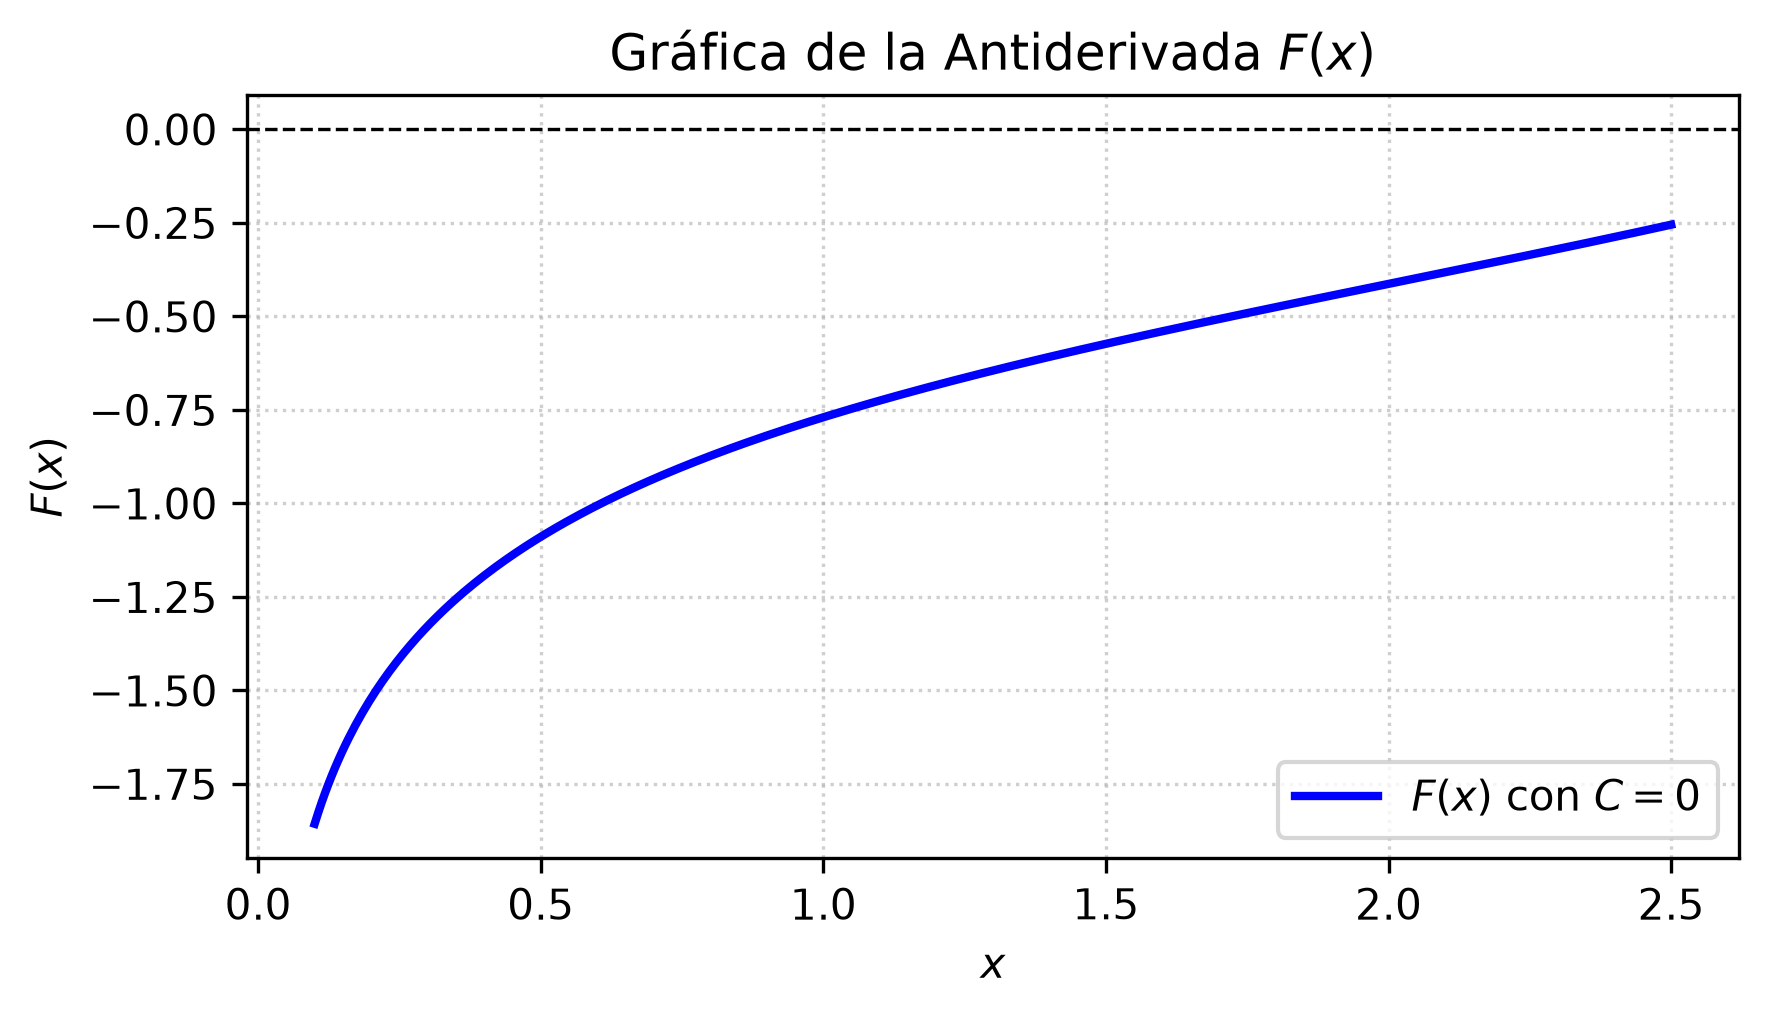
\includegraphics[width=\columnwidth]{semana_04/graficas/SEM04_P12_grafica.png}
	\caption{Representación gráfica de $f(x)$ y su antiderivada $F(x)$ evaluada para la constante de integración $C = 0$ (Problema 12).}
	\label{fig:problema12}
\end{figure}
